\rhead{实验与结果分析}
\chapter{实验与结果分析}

%@@@@@@@@@@@@@@@@@@@@@@@@@@@@
\section{数据集及预处理}
实验所用的所有数据均来自Isobase数据库\cite{park2011isobase}。该数据包含了四种生物的PPI网络数据,每种生物的PPI网络详细信息见表\ref{table:1}。表中的数据是经过预处理的,其中每个PPI网络去除了自环、重边以及独立的节点。Isobase数据库是被普遍使用的生物PPI网络数据库,因此我们选择了这个数据集。


\begin{table}[htbp]
    \centering
    \caption{Isobase数据库关于四种生物的PPI网络数据}
    \label{table:1}
    \begin{tabular}{cccc}
         \hline 物种&点数&边数&平均点度\\
         \hline C.elegans&2974&4827&3.25\\
         D.melanogaster&7387&24937&6.75\\
         H.sapiens&\bf{10296}&54654&10.62\\
         S.cerevisiae&5523&\bf{82656}&\bf{29.93}\\
         \hline
    \end{tabular}
\end{table}

这些都是静态的PPI网络数据,为了构造动态的PPI网络数据,本文使用\cite{zhang2016method}的方法,对每个PPI网络各生成了一个动态PPI网络。为了叙述方便,对这四种生物我们简单的以$ce,dm,hs,sc$来称呼它们。

%@@@@@@@@@@@@@@@@@@@@@@@@@@@@@@@@@
\section{实验方法与环境}
除了本文提出的SGOPT算法,本文还使用了全局匹配算法中的四种经典算法作为和本文算法的对比,分别是IsoRank\cite{singh2008global},SPINAL\cite{aladaug2013spinal},L-GRAAL\cite{malod2015graal}和PROPER\cite{kazemi2016proper}算法。SGOPT算法全部代码由Java构成,并且运行在Linux Ubuntu环境下,详细的环境参数见表\ref{table:2}。

\begin{table}[htbp]
    \centering
    \caption{实验运行环境}
    \label{table:2}
    \begin{tabular}{l|l}
         \hline 
         CPU&Intel Core i7-4790K, 4.00GHz\\
         \hline
         内存&16G\\
         \hline
         操作系统&Linux Ubuntu 14.04LTS,64位\\
         \hline
    \end{tabular}
\end{table}

关于实验中用到的匹配衡量标准,首先是公式\ref{myworkmaxfidefine}的值,为了描述方便,这里简称它为CE(conserved edges)值。因为SGOPT算法的目标就是该公式值的最大化,所以它是我们首要衡量的指标。同时,经过SGOPT算法产生的匹配,我们还会用前文所提到的四个指标去衡量,分别是$EC$,$ISC$,$S^3$和$TWEC$。

%@@@@@@@@@@@@@@@@@@@@@@@@@@@@@@@@@@@@@
\section{关于SGOPT算法的$\alpha,\beta$参数的选择}

正如前文所说的,$\alpha,\beta$作为SGOPT算法的重要参数,太小了可能会导致实验结果变差,太大了则会导致算法耗时,该如何选择一组优秀的参数呢?本文采取了实验确定的办法。

为了描述方便,我们用生物名称1-生物名称2的形式来代表对生物1和生物2的一组实验,即匹配生物1的静态PPI网络和生物2的动态PPI网络,例如$ce-dm$就是匹配$ce$的静态PPI网络与$dm$的动态PPI网络,以此类推。

因为参数$\beta$影响的是每次删掉的匹配数,因此$\beta$越大,一次迭代的时间就越长。但是,$\beta$对匹配效果的影响如何呢?我们希望挑选在同样的时间下,能够产生更好匹配效果的$\beta$参数。因此,我们先给$\alpha$设定一个很大的值,让SGOPT算法可以无限迭代,然后我们选择不同的$\beta$值,让SGOPT算法分别跑$10s,20s,30s,40s,50s,60s$,看看不同的$\beta$参数在同样时间的情况下,产生的匹配的效果。
\begin{figure}[htbp]
\centering
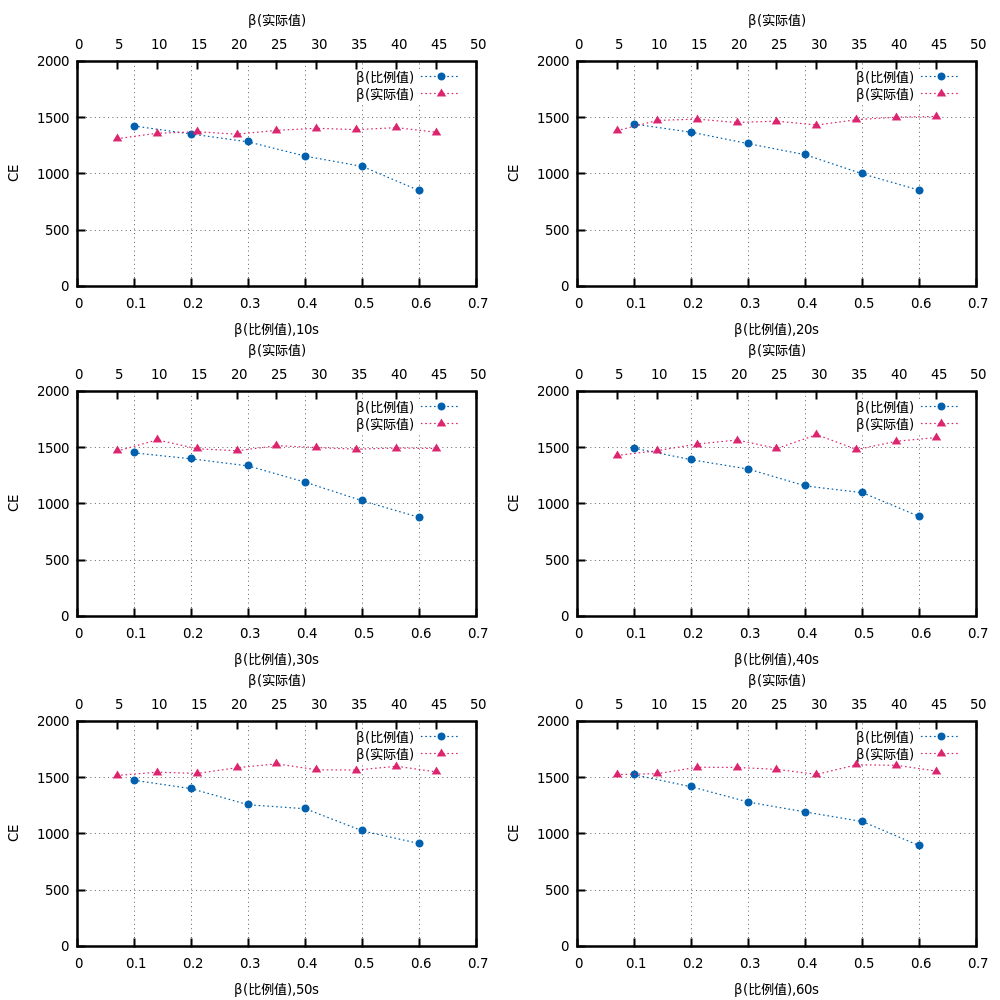
\includegraphics[width=\textwidth]{pic/beta.png}
\caption{SGOPT在不同$\beta$值时运行$10s,20s,30s,40s,50s,60s$的结果} 
\label{fig:beta}
\end{figure}

图\ref{fig:beta}是SGOPT算法在$ce-dm$实验组中优化IsoRank算法的结果。$\beta$(实际值)的意思就是每次迭代时删除的匹配的数目(而不是比例)。蓝色曲线是$\beta$从0.1到0.6变化时SGOPT得到的匹配的结果,从中可以看出,过大的$\beta$意味着每次被删掉的匹配数比较多,需要调整的匹配也越多,一轮的迭代时间会增加,同样的运行时间的情况下,在$\beta$接近0.6的时候,匹配效果明显变差,说明SGOPT不适合$\beta$过大的情况。

而红色曲线表明,每轮迭代时,如果删除的匹配数比较少的情况下,那么SGOPT算法都能很快调整出比较优的解,而且在这种情况下$\beta$稍微大点的效果会比较好。因此我们最终选定$\beta=35$作为SGOPT的参数。

从SGOPT算法中可以看出,每次迭代,匹配的效果不可能变差,所以随着时间的增加,匹配的效果只会越来越好。但是随着时间的推移,能找到更优匹配的概率变得越来越小,因此整个迭代会有一个"收敛"的过程。而$\alpha$参数是迭代次数,也就是时间长短,我们选择$\beta=35$的情况下来运行SGOPT算法,并且记录每轮迭代后当前最优匹配的结果。

\begin{figure}[htbp]
\centering
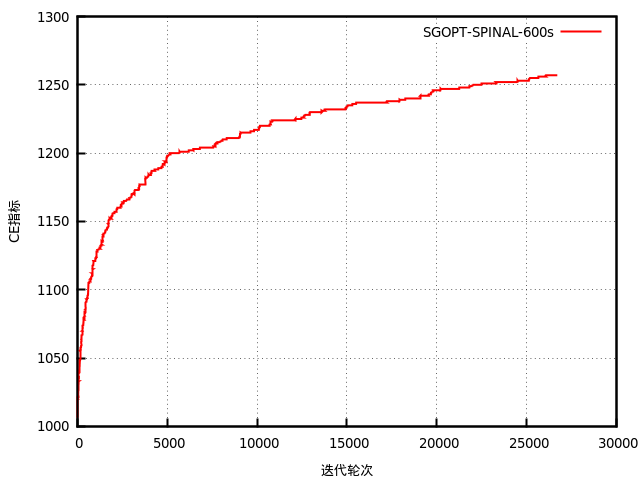
\includegraphics[height=0.4\textheight]{pic/alpha.png}
\caption{SGOPT每轮迭代时的匹配结果(CE)} 
\label{fig:alpha}
\end{figure}

图\ref{fig:alpha}是SGOPT算法在$\beta=35$的情况下,在实验组$ce-dm$上跑了5分钟的的实验结果,可以看到,在前2000轮迭代时,匹配的效果变化十分明显,而2000轮之后,匹配的效果变化开始趋于平缓,说明算法能够得到更优匹配的概率变低了,但是依旧呈上升趋势。

\begin{figure}[htbp]
\centering
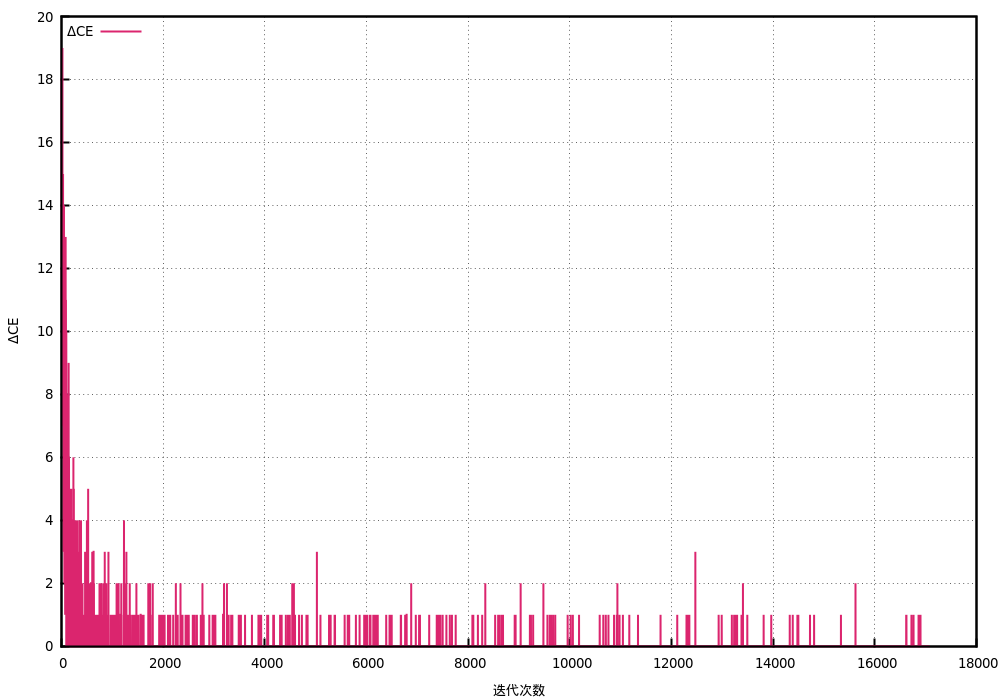
\includegraphics[height=0.4\textheight]{pic/alpha_d.png}
\caption{SGOPT每轮迭代时的匹配结果$(\Delta CE)$} 
\label{fig:alpha_d}
\end{figure}

图\ref{fig:alpha_d}是图\ref{fig:alpha}关于$\Delta CE$值的实验结果。从中大概可以看出,在迭代2000次以后,每次更新最优匹配的时候,$CE$值增幅基本只在1,2跳动,偶尔能够有3的增幅,并且随着迭代次数的增加,这样的增幅变得越来越少(空隙越来越大)。因此,我们设定$\alpha=14000$作为之后实验的参数。

而且,结合图\ref{fig:beta}也可以看出,$\beta=35$的情况下,算法运行$60s$之后,$CE$值就超过了1500,而这正是图\ref{fig:alpha}中大约迭代次数为2000左右的时候。所以SGOPT算法可以大约在1分钟左右就能找到非常优的解了。

%@@@@@@@@@@@@@@@@@@@@@@@@@@@@@@@@@@@@@@@@@
\section{不同算法之间的比较}

确定了$\alpha,\beta$参数以后,接下来的实验就是SGOPT算法与其他算法的比较。我们分别做了$ce-dm,ce-hs,cs-sc,dm-hs,dm-sc,hs-sc$六组实验,每组实验都先用4种静态PPI网络匹配算法,求得初始匹配$f$,然后以$f$为基础匹配运行SGOPT算法,最终得到新的匹配。

四种静态匹配算法的运行参数见表\ref{table:3}。

\begin{table}[htbp]
    \centering
    \caption{静态匹配与运行参数}
    \label{table:3}
    \begin{tabular}{ccc}
         \hline 算法&命令行&参数\\
         \hline IsoRank&-alpha $\alpha$ -I 50&$\alpha=1$\\
         SPINAL&-II -alpha $\alpha$&$\alpha=1$\\
         L-GRAAL&-alpha $\alpha$&$\alpha=1$\\
         PROPER&$-l$ $l$ $-r$ $r$&$l=500,r=1$\\
         \hline
    \end{tabular}
\end{table}

图\ref{fig:all}为SGOPT算法与其他四种静态匹配算法的比较结果。横坐标表示实验组,纵坐标是匹配结果,可以看出,四种静态算法在动态PPI网络上的匹配结果各有好坏,IsoRank的结果是最差的,而L-GRAAL的结果则比起其他三种算法都要好。SPINAL和PROPER则没有明显的效果差别。而SGOPT的柱状图表示,对于已有的四种静态匹配算法,SGOPT都能在它们已有的匹配上改良它们的匹配效果,产生效果更好的匹配。从中可以看出SGOPT有明显的优势。

值得一提的是,虽然IsoRank在动态PPI网络上的匹配效果非常糟糕,但是经过SGOPT改良后的匹配,效果甚至高于L-GRAAL经过SGOPT改良后的匹配,这可能是因为糟糕的匹配给了SGOPT更多调整的机会与空间,使得SGOPT能够从全局的角度上来优化整个匹配,从而产生了更优秀的匹配结果。

\begin{figure}[htbp]
\centering
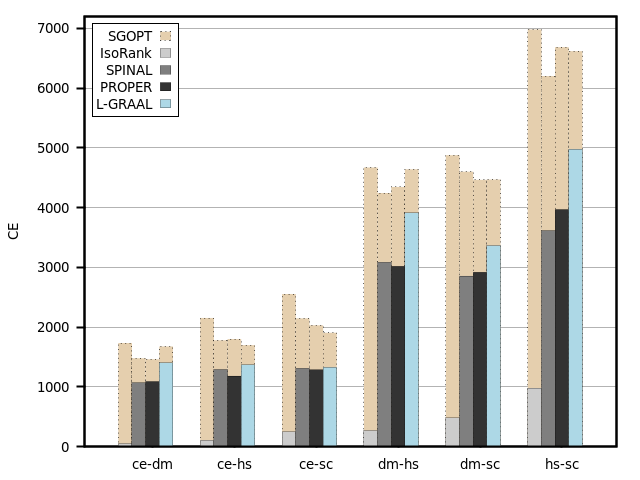
\includegraphics[height=0.4\textheight]{pic/all.png}
\caption{SGOPT与其他四种算法的结果比较} 
\label{fig:all}
\end{figure}

图\ref{fig:all_improve}展示了SGOPT对于其他四种算法已有匹配的效果的提高程度,即
\begin{equation}
\frac{\text{提高后的CE值-提高前的CE值}}{\text{提高前的CE值}}    
\end{equation}
可以看到SGOPT对于提高IsoRank的匹配有明显的效果。而对于其他四种算法的提高,SPINAL和PROPER能够达到40\%~60\%,而对于L-GRAAL算法效果的提高则稍微差一点,为20\%~40\%左右。然而总体上来说,有这种结果已经说明了SGOPT具有的优势。

\begin{figure}[htbp]
\centering
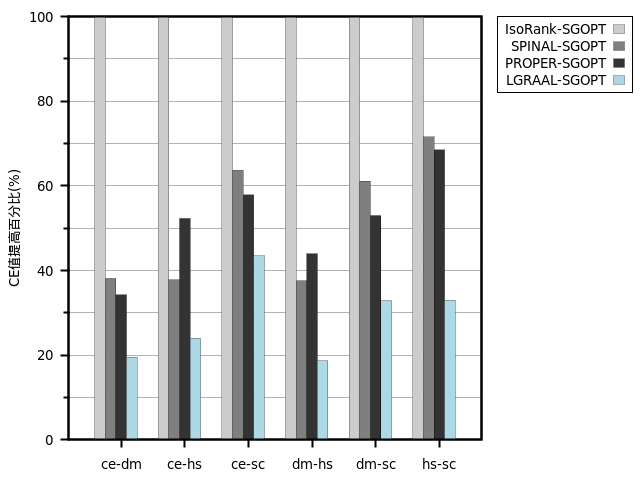
\includegraphics[height=0.4\textheight]{pic/all_improve.png}
\caption{SGOPT相比其他四种算法提高的程度} 
\label{fig:all_improve}
\end{figure}

%@@@@@@@@@@@@@@@@@@@@@@@@@@@@@@@@@@@@@2
\section{EC,ICS,$S^3$,TWEC指标的对比}
目前为止所有的实验采用的指标都是$CE$值,那么在另外的指标下,SGOPT算法的效果又如何呢?图\ref{fig:other}是所有六组实验下,用SGOPT算法求得的各项指标,与优化前静态匹配得到的指标的对比。可以看到,SGOPT对于IsoRank的优化依旧非常明显,这是因为IsoRank效果太糟糕的缘故。而除了IsoRank,SGOPT在大部分情况下对于4项指标都能产生很好的优化效果,而且和图\ref{fig:all_improve}相似的,在SPINAL和PROPER的优化上相差不多,而对于L-GRAAL的优化则相对较差。另外值得一提的便是优化呈负效果的那些情况。

\begin{figure}[htbp]
\centering
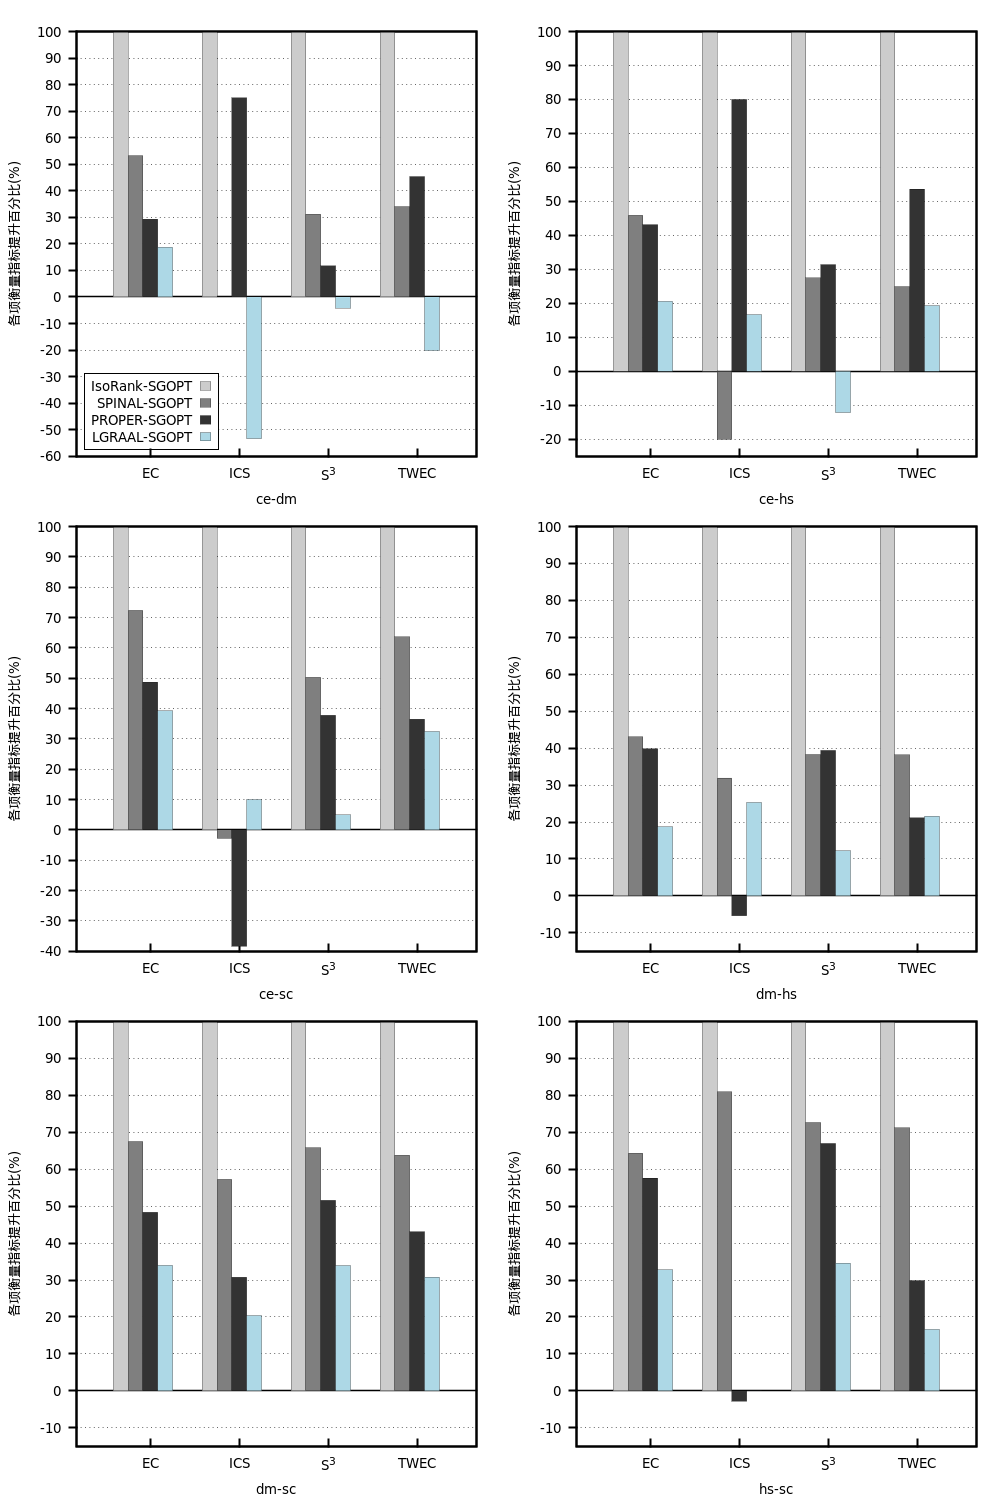
\includegraphics[width=\textwidth]{pic/other.png}
\caption{SGOPT相比其他四种算法在EC,ICS,$S^3$,TWEC指标上提高的程度} 
\label{fig:other}
\end{figure}

由EC值的公式定义\ref{myworkecdefine}可知,其正比于CE值,由于SGOPT优化的便是CE值,所以在所有实验中,EC指标肯定都可以得到优化。

而由ICS和$S^3$的公式定义\ref{myworkicsdefine}, \ref{myworks3define}可知,指标不仅和源网络有关,和目标网络也有关,而在目标网络是动态的情况下,优化CE值不一定能带动这两项指标的增长。实验也反应了这个情况,在前三组实验中,ICS在后面三种算法的优化上有时会达到负的优化效果,这样的情况出现了5次,而$S^3$则相对较好,只出现了2次。后三组试实验中,情况则比较乐观。

理论上看,SGOPT算法的目的是优化CE值,而CE值越大,意味着源网络有更多的边被保留在了目标网络中,因此对于EC这个只考虑源网络结构的指标,有很好的优化效果。而ICS是只考虑目标网络结构的指标,着重衡量目标网络中被匹配边的稀疏程度,而不是源网络,所以在目标网络是稠密网络的情况下,以优化CE值为目的的SGOPT算法对于这个ICS这个指标比较敏感,时好时坏。而剩下的$S^3$和TWEC指标,则同时考虑了源网络和目标网络,因此相对于ICS指标来说,更具有综合意义。而且SGOPT对于这两个指标的敏感程度,明显没有ICS来得高,从实验结果中也可以看到。


